\documentclass[letterpaper,10pt]{article}
\usepackage{graphicx}
\usepackage[margin=2cm]{geometry}
\usepackage{url}
\usepackage{listings}

\title{Testing Software Installation}
\author{44-671: Streaming Data}
\date{}

\begin{document}
\maketitle

\begin{enumerate}
	\item Complete the installation of Docker and download the required files from the course website.  Put the \texttt{.yml} file in a directory you can easily find (I chose \texttt{Documents/streaming-data})
	\item Open a terminal window in the directory you downloaded the \texttt{docker-compose.yml} file
		\begin{itemize}
			\item Windows quicktip: go to the folder in the file explorer, type \texttt{powershell} in the address bar, and hit enter
		\end{itemize}
	\item Run the command \texttt{docker-compose up} (type the command in the terminal and hit enter)
		\begin{itemize}
			\item Note: On Windows and MacOS, you'll be able to start the service through Docker Desktop for future assignments; you will be provided more information on how to start and stop the services when necessary
		\end{itemize}
	\item Open a web browser and navigate to \url{http://localhost:8888/lab}
		\begin{itemize}
			\item Note: the Docker containers are designed to not require a username/password or token.  This is not a secure practice; it is recommended you only have the docker application started when doing assignments and stop the application when you are finished.
		\end{itemize}
	\item You should see a window that looks like this:
		\begin{center}
			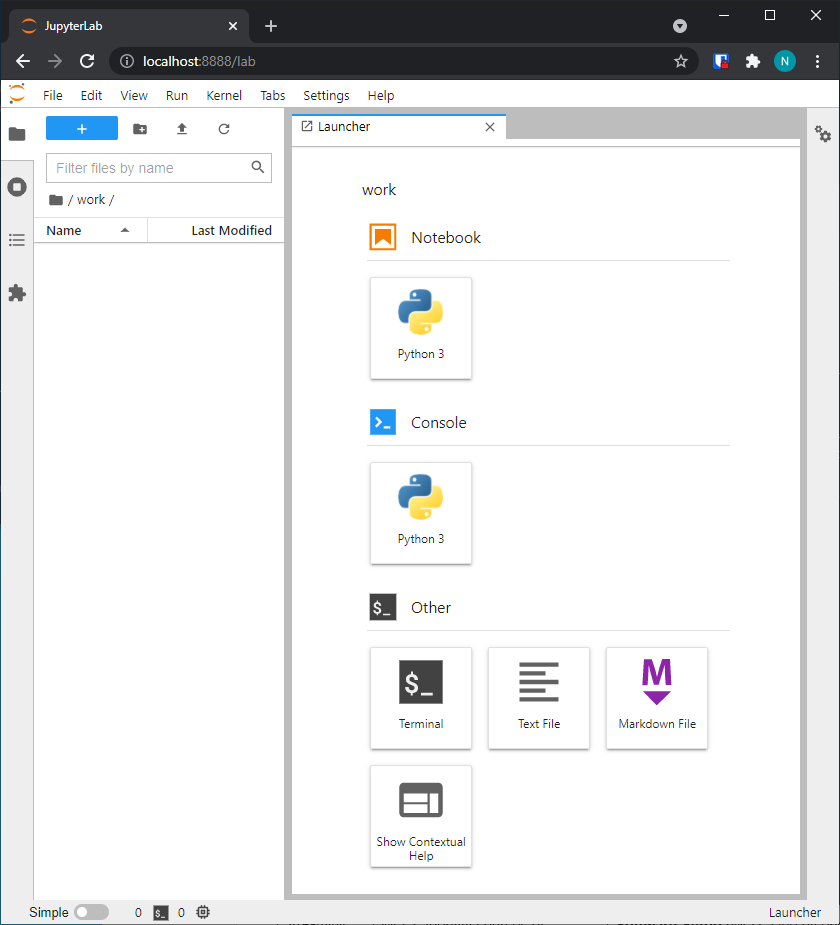
\includegraphics[width=0.5\textwidth]{jupyterlab.PNG}
		\end{center}
		\begin{itemize}
			\item Note: you may see other files in the left hand pane; that is acceptable as they may be used later in the course
		\end{itemize}
	\item In the right hand pane, under "Notebook" select the Python 3 Button.  You should be greeted with a window that looks like this:
		\begin{center}
			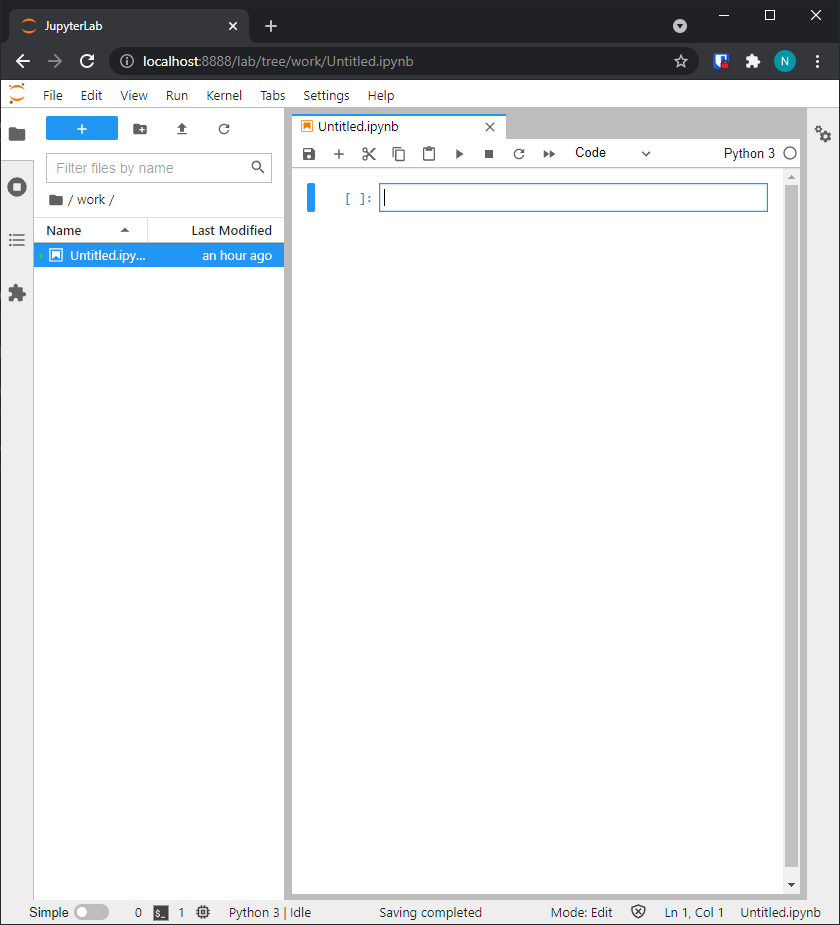
\includegraphics[width=0.5\textwidth]{new_notebook.PNG}
		\end{center}
	\item The top box in the right hand pane is a \emph{cell}; we will create multiple cells in Python notebooks through the duration of this course.  In the top cell write the following code (type it out; do NOT copy and paste):
		\begin{lstlisting}[language=Python]
			print('Hello world!')
			print('My name is <name>')
		\end{lstlisting}
		but replace \texttt{<name>} with your name.  Run the cell either by pressing the triangle button at the top of the screen or by holding Shift and pressing Enter.  The result should look similar to:
		\begin{center}
			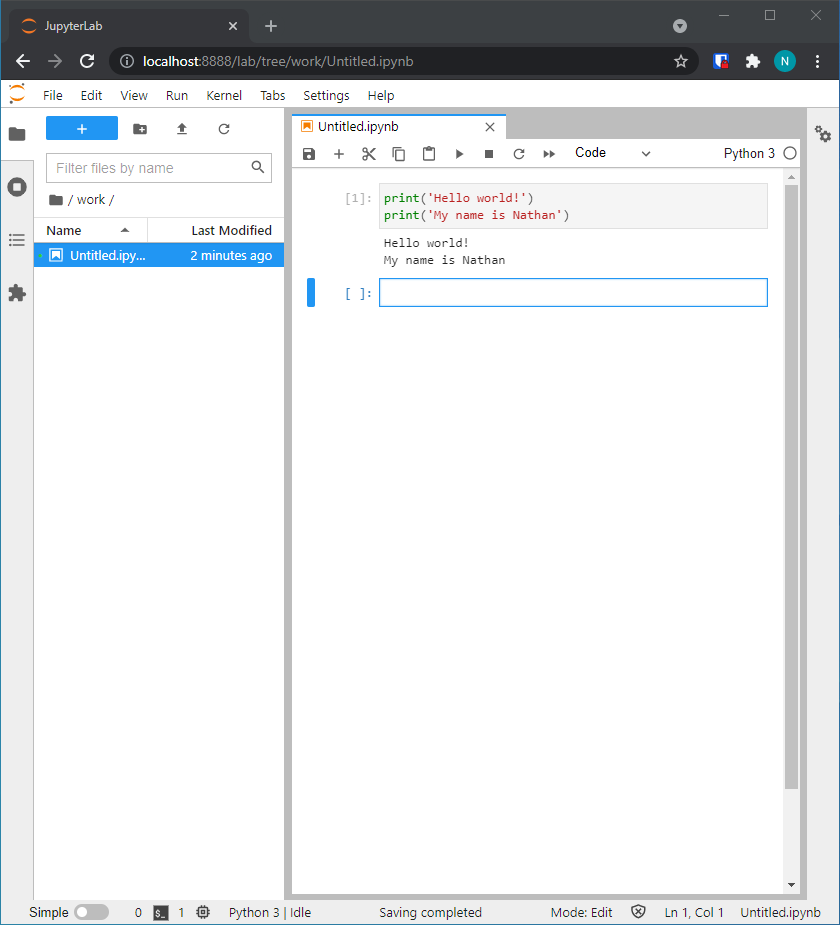
\includegraphics[width=0.8\textwidth]{hello_world.PNG}
		\end{center}
	\item Determine the name of your RabbitMQ instance
		\begin{itemize}
			\item Windows/MacOS: Open Docker Desktop, navigate to the Containers/Apps tab.  You should see an app running (it may have a different name different for you)
				\begin{center}
					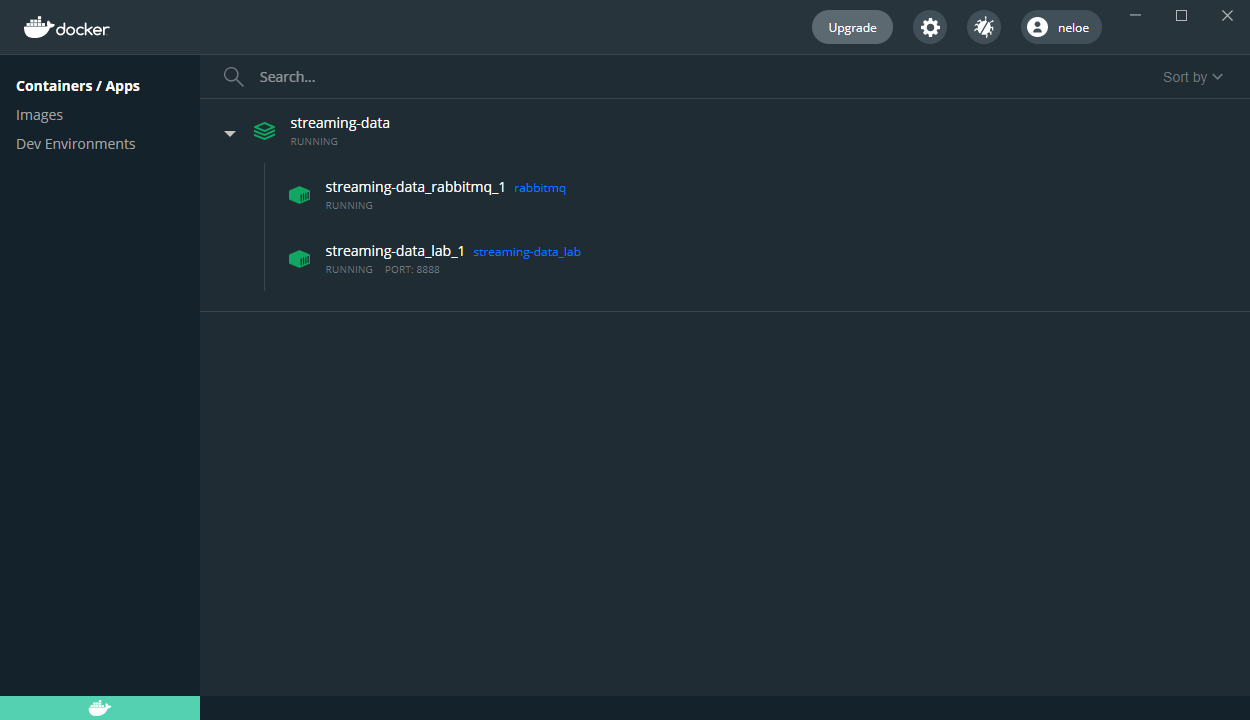
\includegraphics[width=0.9\textwidth]{docker-desktop.PNG}
				\end{center}
			\item Linux: Run \texttt{docker-compose ps} from the directory containing the \texttt{docker-compose.yml} file.  You should see output like:
				\begin{center}
					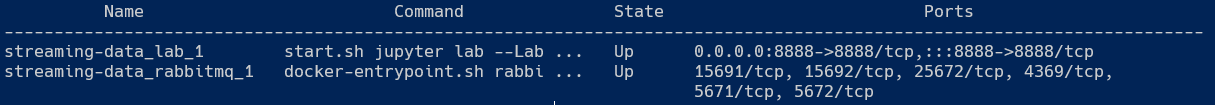
\includegraphics[width=0.9\textwidth]{docker-compose-ps.PNG}
				\end{center}
		\end{itemize}
		For me, the RabbitMQ instance is named \texttt{streaming-data\_rabbitmq\_1}; your name may differ.  Use the instance name you see on your computer for the next step.
	\item In the new cell that was created at the bottom of the python notebook, write the following code (substituting \texttt{localhost} with the hostname you determined in the previous step:
		\begin{lstlisting}[language=Python]
import pika

connection = pika.BlockingConnection(pika.ConnectionParameters('localhost'))
channel = connection.channel()
print('Connection completed')
		\end{lstlisting}
		Run the cell as you did above.  The resulting output should look like (I closed the files tab so you could see all of the code):
		\begin{center}
			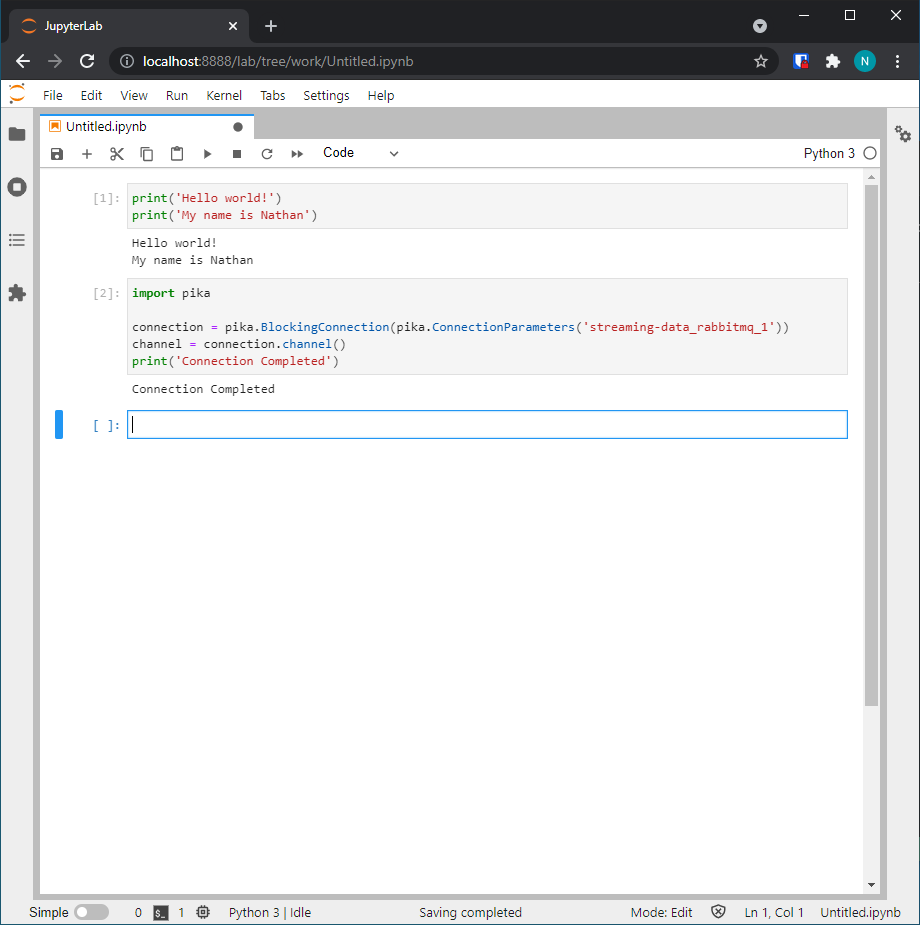
\includegraphics[width=0.9\textwidth]{successful-connect.PNG}
		\end{center}
		If all goes well, you should get no errors (usually highlighted in red) and the message ``Connection Completed''.  If you receive errors use your favorite search engine or contact your instructor to help in troubleshooting.
	\item Export your notebook: In the file tab in JupyterLab, go to ``Export Notebook As...'' and choose PDF.  It should download a file (possibly named \texttt{Untitled.pdf} unless you changed the name of the notebook.  Ensure that the contents of the PDF look like the code on your screen and submit the PDF to the course website.
		\begin{center}
			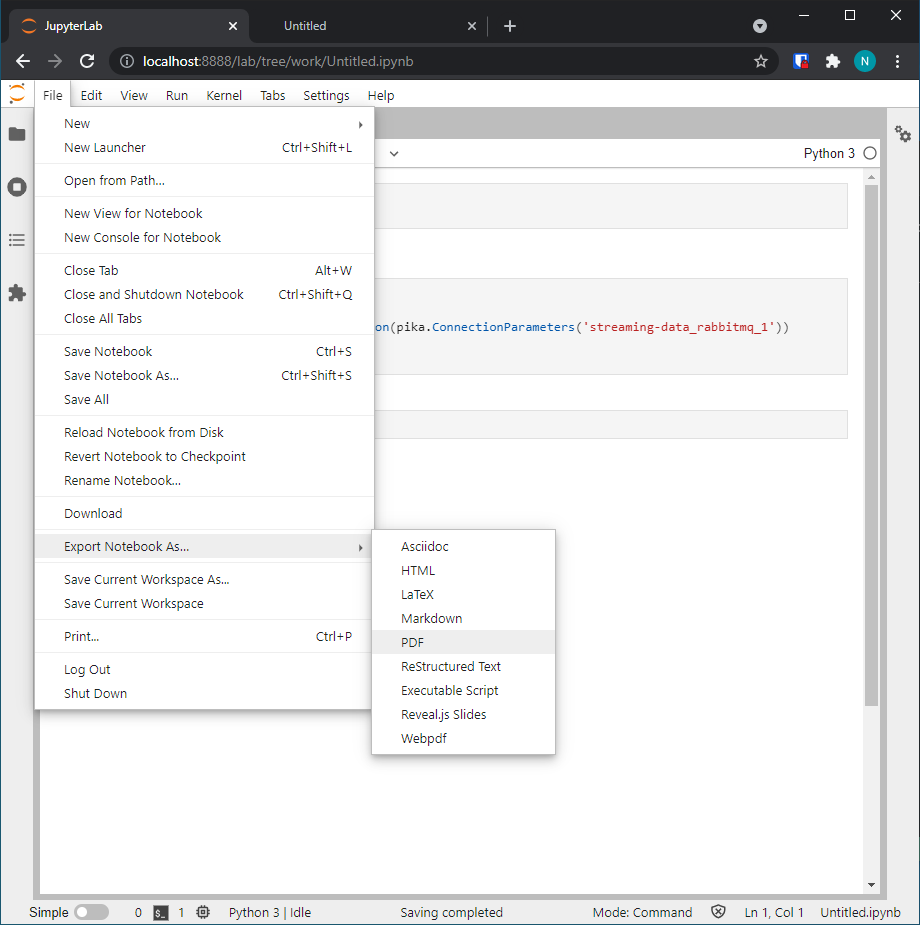
\includegraphics[width=0.9\textwidth]{export.PNG}
		\end{center}
\end{enumerate}

\end{document}
